
\section{附錄一、安裝與設定}

在學習程式語言之前,要先設定好程式的開發環境。這個章節會教同學如何安裝及設定開發環境。首先,說明如何安裝兩套軟體「Code::Blocks」以及「瘋狂程設」;再來,說明如何註冊瘋狂程設的帳號;最後,說明如何使用瘋狂程設。

\subsection{安裝CodeBlocks}
%\subsubsection{步驟一:下載}
	在Google搜尋輸入關鍵字「codeblocks」,選擇搜尋結果「Download binary - Code::Blocks」。也可以直接輸入以下網址 \url{http://www.codeblocks.org/downloads/26},參考\autoref{install001}。
	\begin{figure}[H]
		\centering
		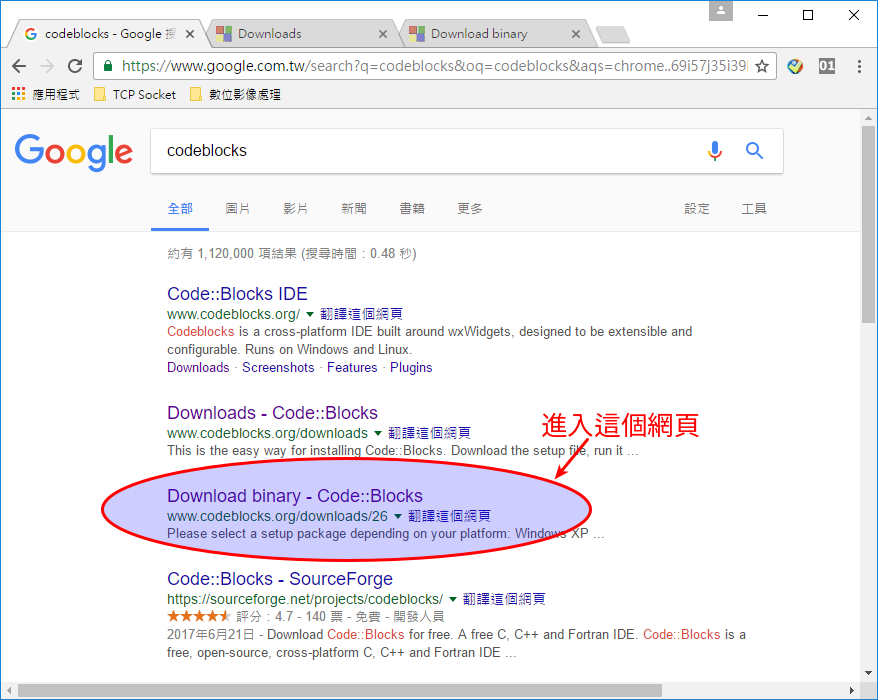
\includegraphics[width=0.8\textwidth]{fig/install_and_setting/install_001_searchCodeblocks}
		\caption{codeblocks搜尋結果}
		\label{install001}
	\end{figure}

\newpage
	進入官網下載頁面後,選擇包含mingw-setup的檔案,點選該檔案右邊的連結下載,參考\autoref{install002}。
	\begin{figure}[H]
		\centering
		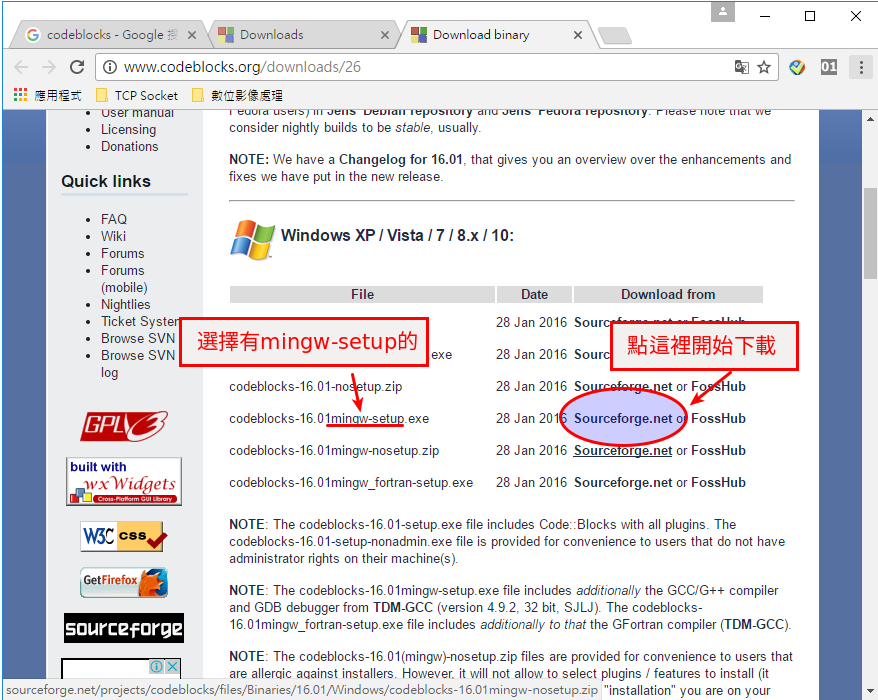
\includegraphics[width=0.8\textwidth]{fig/install_and_setting/install_002_Download_binary}
		\caption{Download binary頁面}
		\label{install002}
	\end{figure}
	
	找到剛剛下載的安裝檔codeblocks-16.01mingw-setup.exe,點兩下開啟安裝精靈,參考\autoref{install003}。
	\begin{figure}[H]
		\centering
		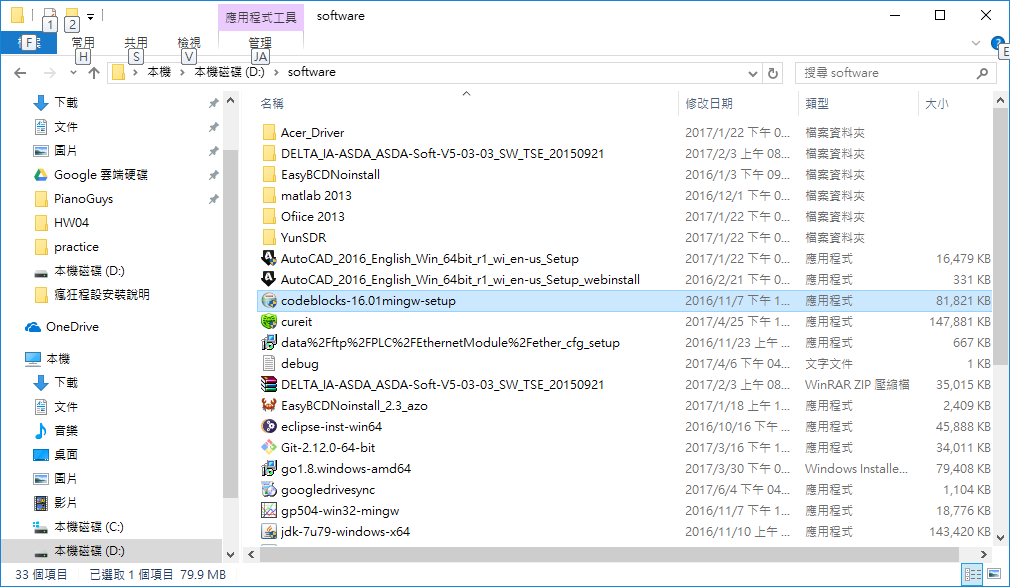
\includegraphics[width=0.8\textwidth]{fig/install_and_setting/install_003_openEXE}
		\caption{點兩下開啟CodeBlocks安裝檔}
		\label{install003}
	\end{figure}
	
	\newpage
	請不要修改安裝精靈的任何設定,只要一直點「Next」就好。絕對不可以更改檔案路徑,參考\autoref{install004}。
		\begin{figure}[H]
			\centering
			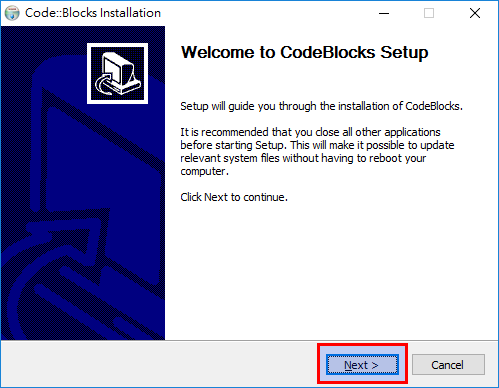
\includegraphics[width=0.8\textwidth]{fig/install_and_setting/install_004_setup01}
			\caption{啟動安裝精靈,點「Next」}
			\label{install004}
		\end{figure}
	
		\begin{figure}[H]
			\centering
			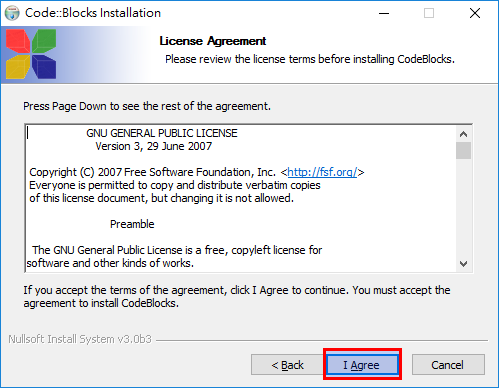
\includegraphics[width=0.8\textwidth]{fig/install_and_setting/install_005_setup02}
			\caption{點「I Agree」}
		\end{figure}
			
		\begin{figure}[H]
			\centering
			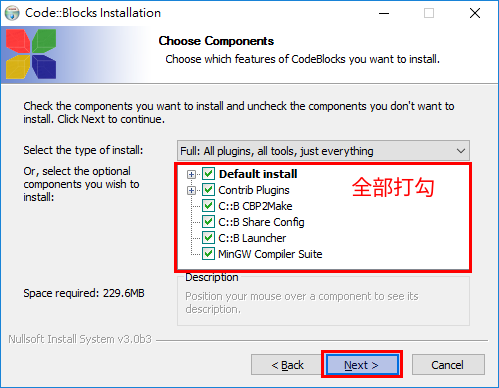
\includegraphics[width=0.8\textwidth]{fig/install_and_setting/install_006_setup03}
			\caption{全部打勾,點「Next」}
		\end{figure}
	
		\begin{figure}[H]
			\centering
			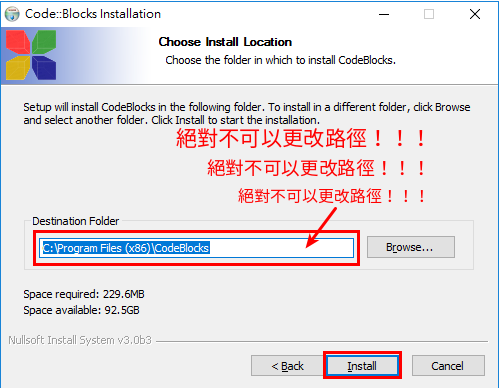
\includegraphics[width=0.8\textwidth]{fig/install_and_setting/install_007_setup04}
			\caption{直接點「Install」,絕對不可以更改路徑}
		\end{figure}

		\begin{figure}[H]
			\centering
			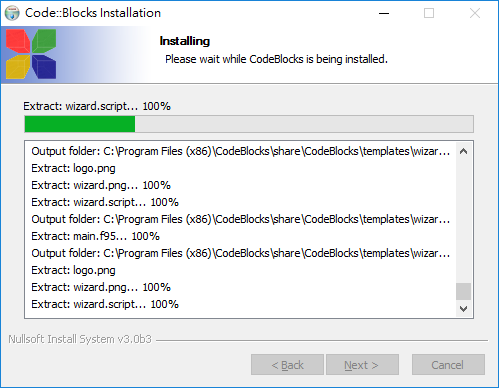
\includegraphics[width=0.8\textwidth]{fig/install_and_setting/install_008_setup05}
			\caption{正在安裝,請耐心等待}
		\end{figure}
		
		\begin{figure}[H]
			\centering
			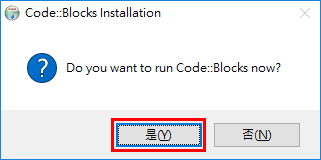
\includegraphics[width=0.8\textwidth]{fig/install_and_setting/install_009_setup06}
			\caption{點「是(Y)」,起動codeBlocks}
		\end{figure}
		
		\begin{figure}[H]
			\centering
			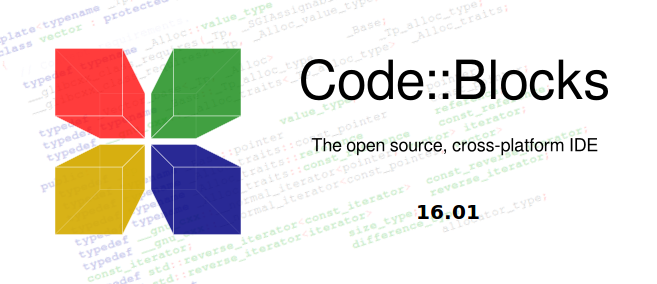
\includegraphics[width=0.8\textwidth]{fig/install_and_setting/install_010_setup07}
			\caption{正在開啟Codeblocks}
		\end{figure}
		
		\begin{figure}[H]
			\centering
			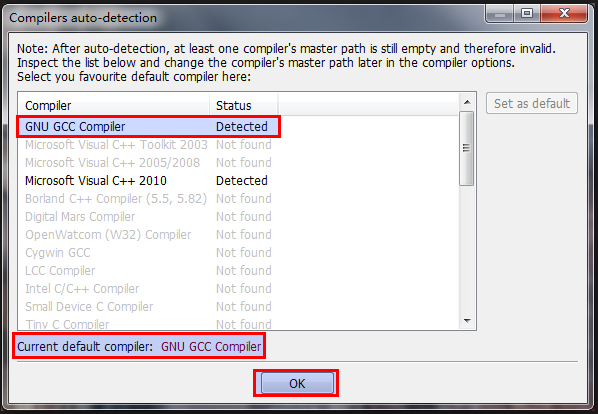
\includegraphics[width=0.8\textwidth]{fig/install_and_setting/install_011_setup08}
			\caption{確定有偵測到 GNU GCC Compiler,點「OK」}
		\end{figure}
		
		\begin{figure}[H]
			\centering
			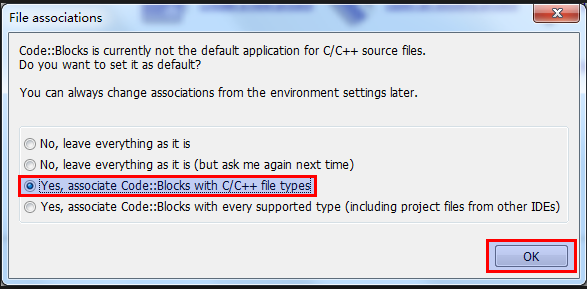
\includegraphics[width=0.8\textwidth]{fig/install_and_setting/install_012_setup09}
			\caption{選第三個,將CodeBlocks設為開起程式碼的預設程式}
		\end{figure}
		
		\begin{figure}[H]
			\centering
			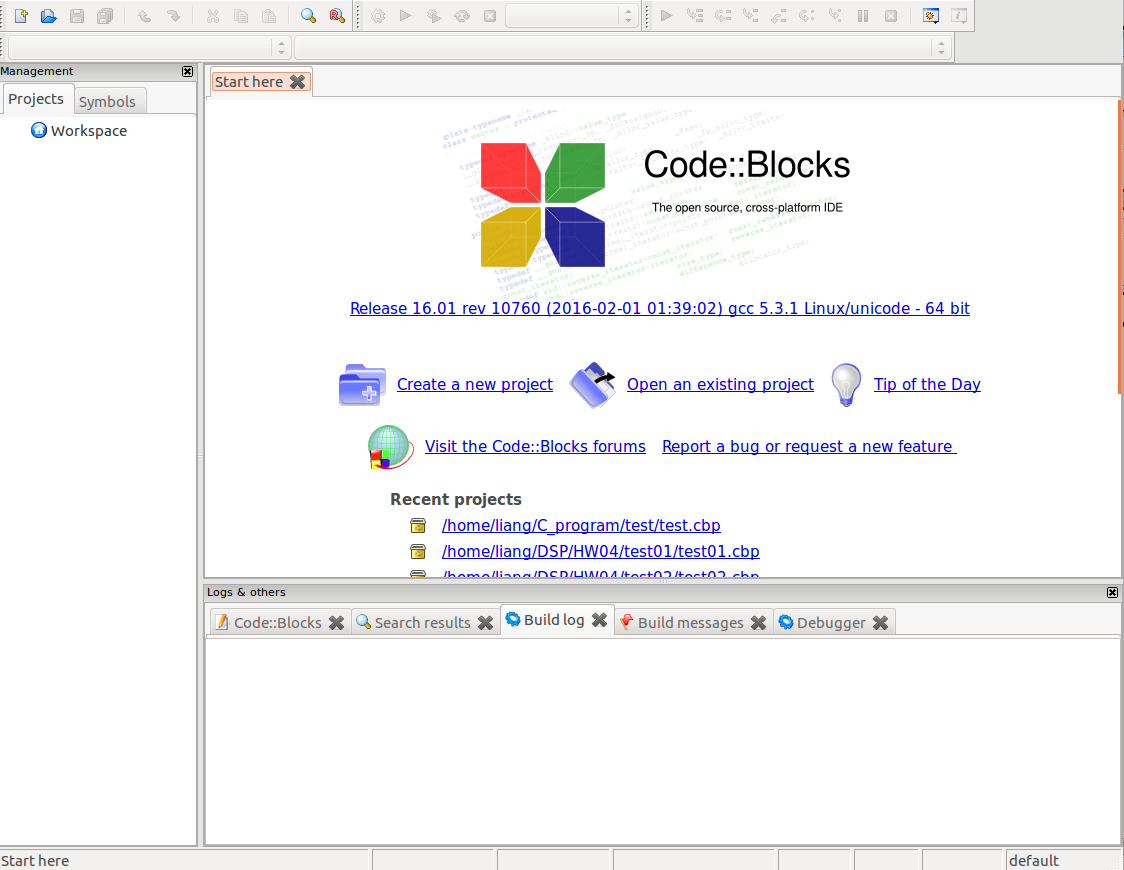
\includegraphics[width=0.8\textwidth]{fig/install_and_setting/install_013_setup10}
			\caption{成功開啟CodeBlocks}
		\end{figure}
		
		\begin{figure}[H]
			\centering
			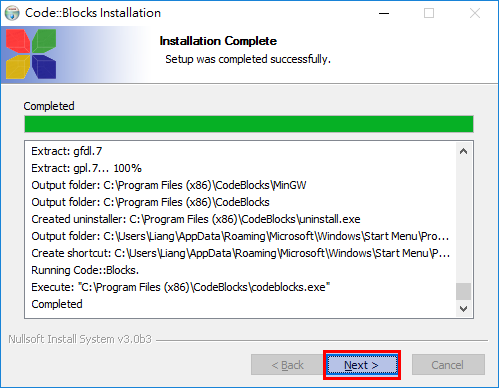
\includegraphics[width=0.8\textwidth]{fig/install_and_setting/install_014_setup11}
			\caption{回到安裝精靈,點「Next」}
		\end{figure}
		
		\begin{figure}[H]
			\centering
			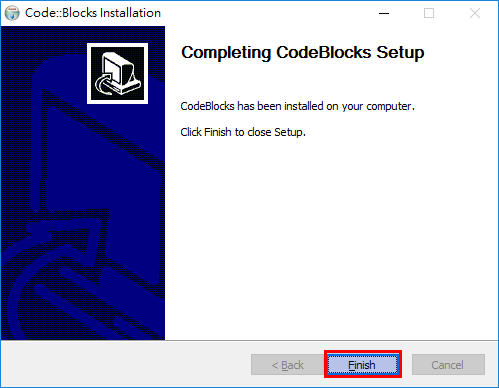
\includegraphics[width=0.8\textwidth]{fig/install_and_setting/install_015_setup12}
			\caption{點「Finish」,關閉安裝精靈}
		\end{figure}
	
\subsection{安裝「瘋狂程設」}
在google瀏覽器上搜尋關鍵字「瘋狂程設」,進入「瘋狂程設:自動閱卷的程式設計機上考試題庫暨考試系統」網站。也可以直接輸入網址:\url{http://coding-frenzy.arping.me/},參考\autoref{install016}。
		\begin{figure}[H]
			\centering
			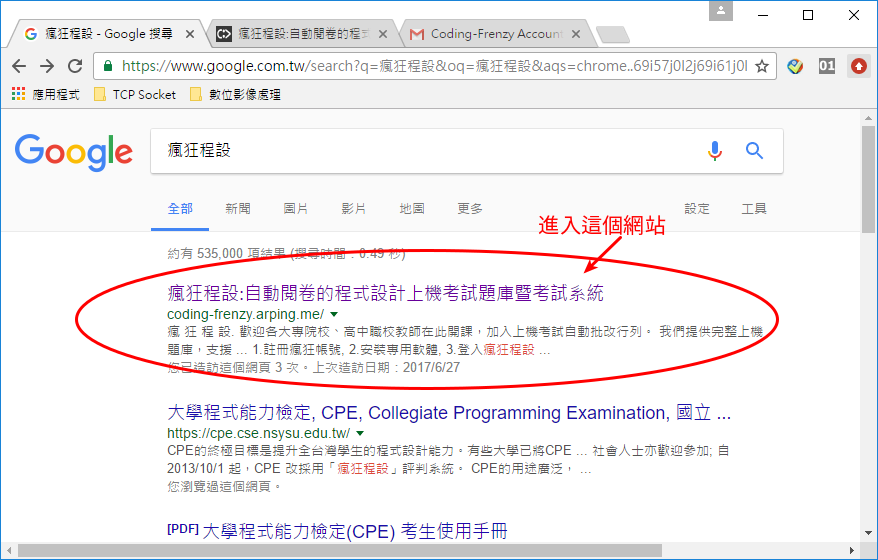
\includegraphics[width=0.8\textwidth]{fig/install_and_setting/install_016}
			\caption{「瘋狂程設」搜尋結果}
			\label{install016}
		\end{figure}
		進入瘋狂程設首頁後,點下方的「2.安裝專用軟體」,參考\autoref{install017}及\autoref{install018}。
		\begin{figure}[H]
			\centering
			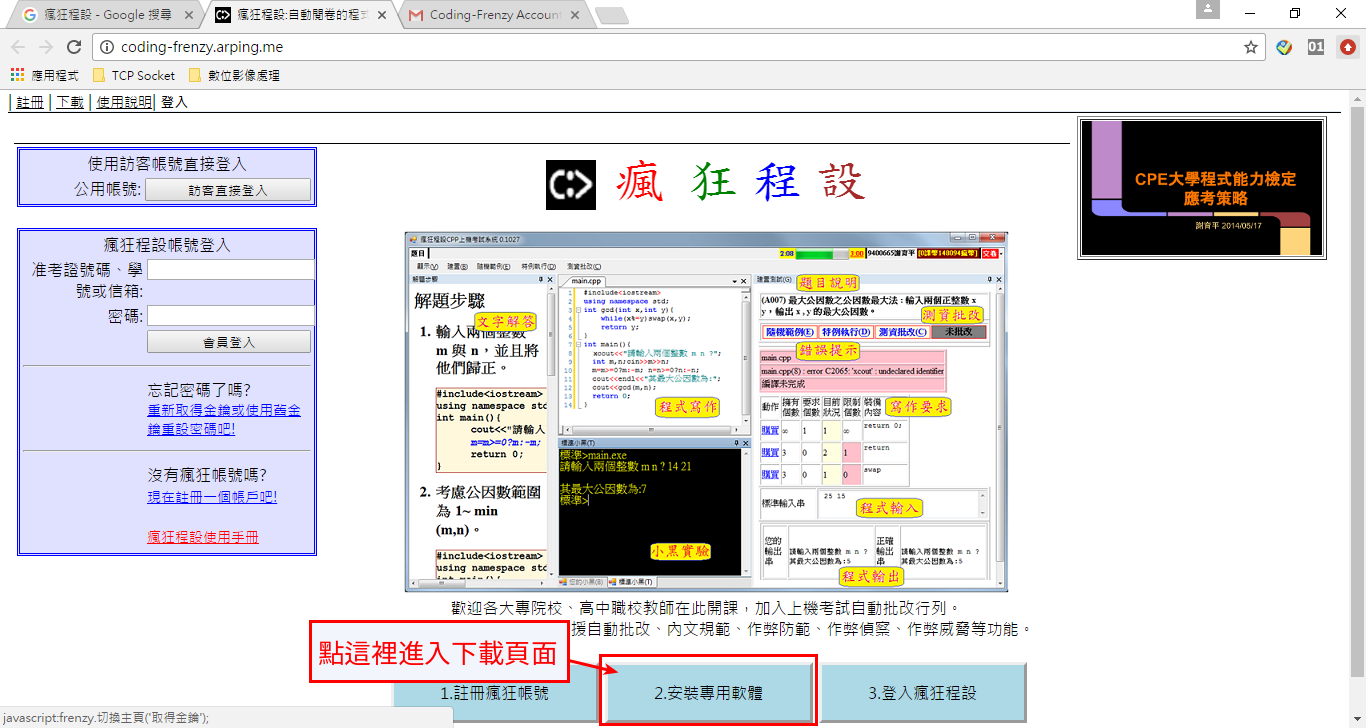
\includegraphics[width=0.8\textwidth]{fig/install_and_setting/install_017}
			\caption{瘋狂程設首頁}
			\label{install017}
		\end{figure}
		
		\begin{figure}[H]
			\centering
			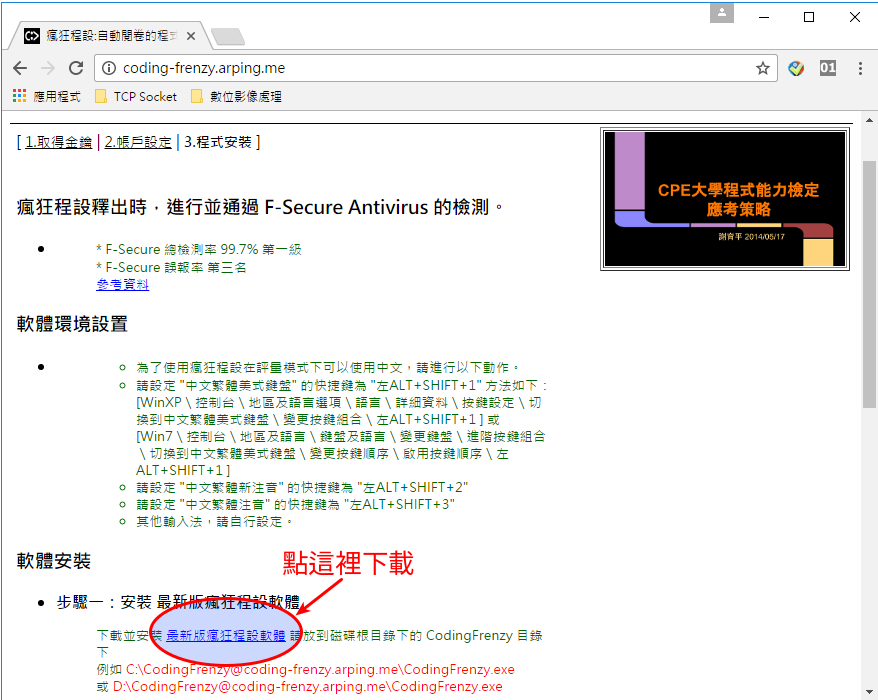
\includegraphics[width=0.8\textwidth]{fig/install_and_setting/install_018}
			\caption{下載頁面}
			\label{install018}
		\end{figure}
		
		 請將剛才下載的壓縮檔複製到C槽裡,直接放在根目錄C下面,然後解壓縮。對zip檔按「右鍵」 -> 解壓縮到CodingFrenzy@coding-frenzy.arping.me\textbackslash,參考\autoref{install019}。
		\begin{figure}[H]
			\centering
			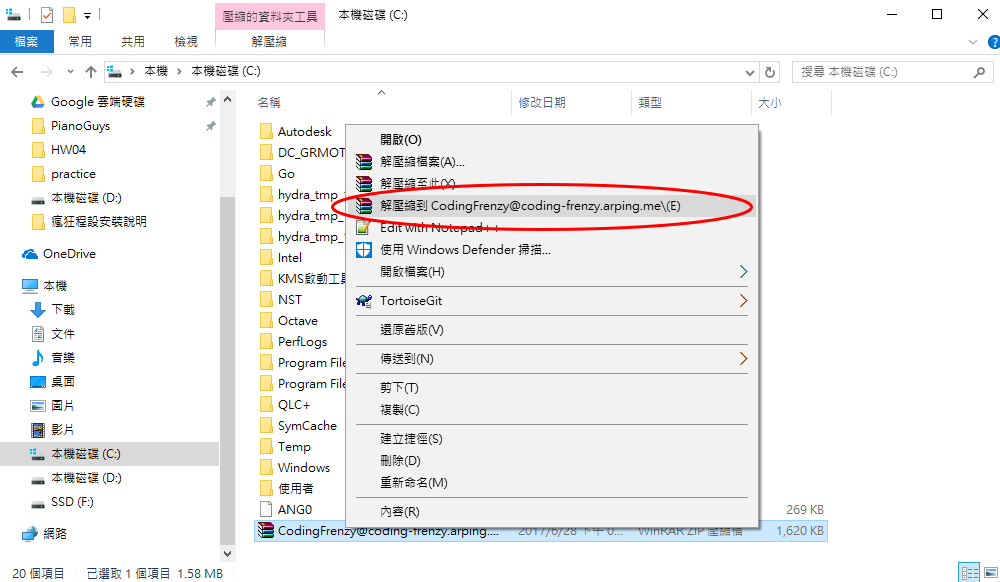
\includegraphics[width=0.8\textwidth]{fig/install_and_setting/install_019}
			\caption{右鍵 -> 解壓縮到CodingFrenzy@coding-frenzy.arping.me\textbackslash}
			\label{install019}
		\end{figure}
		
		\newpage
		之後,C槽裡面會出現一個資料夾「CodingFrenzy@coding-frenzy.arping.me」,點開此資料夾,參考\autoref{install020}。
		\begin{figure}[H]
			\centering
			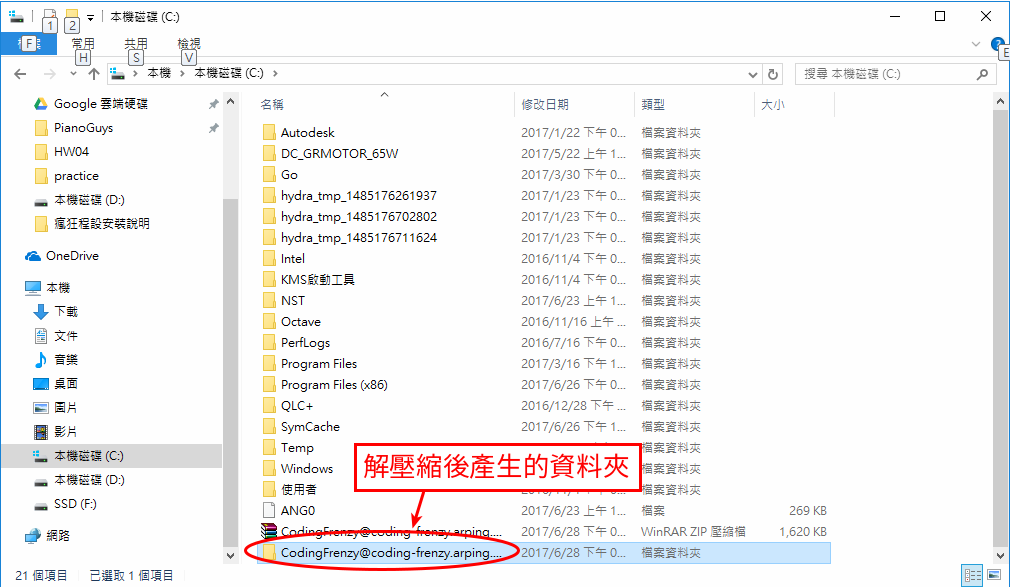
\includegraphics[width=0.8\textwidth]{fig/install_and_setting/install_020}
			\caption{點開解壓縮後的資料夾}
			\label{install020}
		\end{figure}
		\begin{figure}[H]
			\centering
			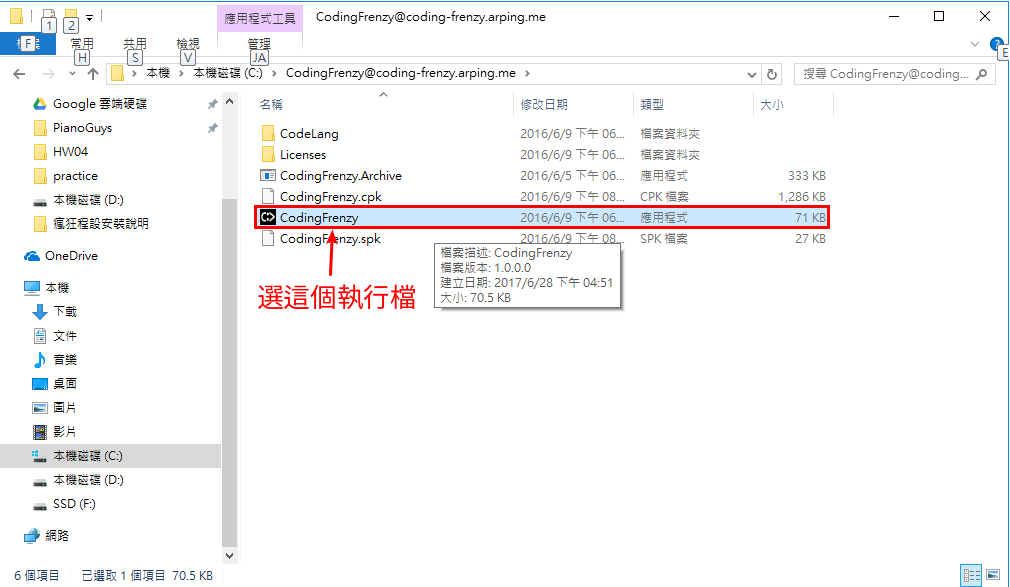
\includegraphics[width=0.8\textwidth]{fig/install_and_setting/install_021}
			\caption{開啟CodingFrenzy執行檔}
		\end{figure}
		\begin{figure}[H]
			\centering
			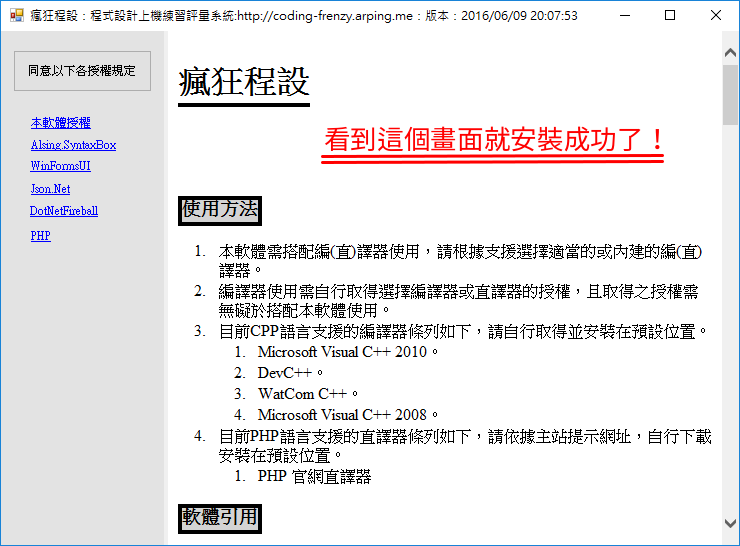
\includegraphics[width=0.8\textwidth]{fig/install_and_setting/install_022}
			\caption{安裝成功}
		\end{figure}

		回到資料夾裡,會多出一些東西,不用理它們。對CodingFrenzy.exe執行檔按「右鍵」-> 「傳送到」 -> 「桌面(建立捷徑)」,參考\autoref{install023}。
		\begin{figure}[H]
			\centering
			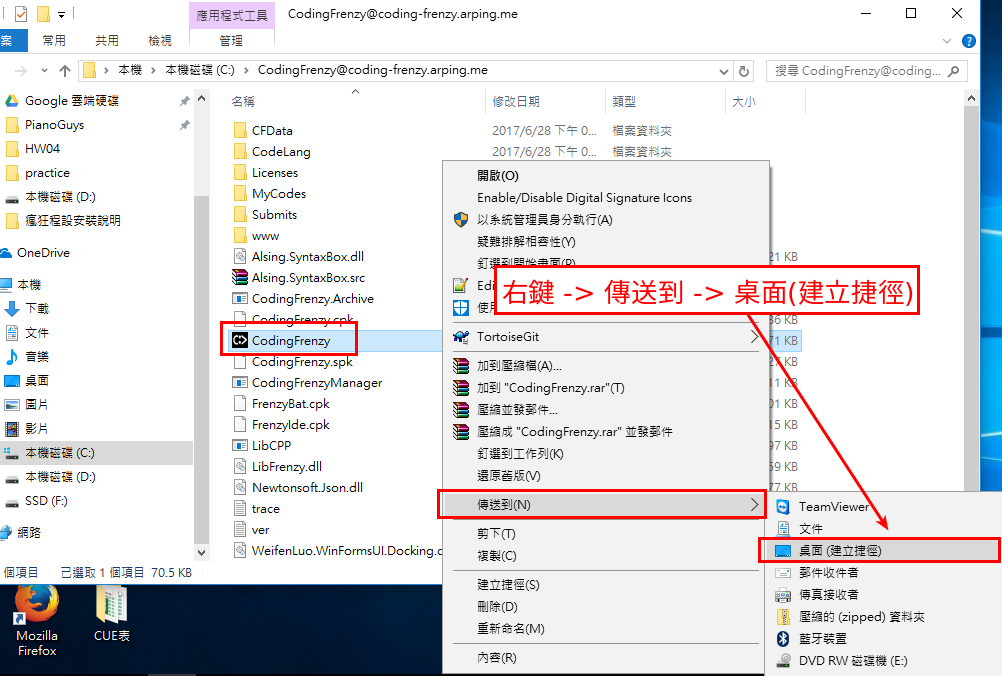
\includegraphics[width=0.8\textwidth]{fig/install_and_setting/install_023}
			\caption{建立桌面捷徑}
			\label{install023}
		\end{figure}
	
	\newpage
		按鍵盤「win+D」切換到桌面,找到CodingFrenzy桌面捷徑,以後就可以從這邊直接執行瘋狂程設了,參考\autoref{install024}。
		\begin{figure}[H]
			\centering
			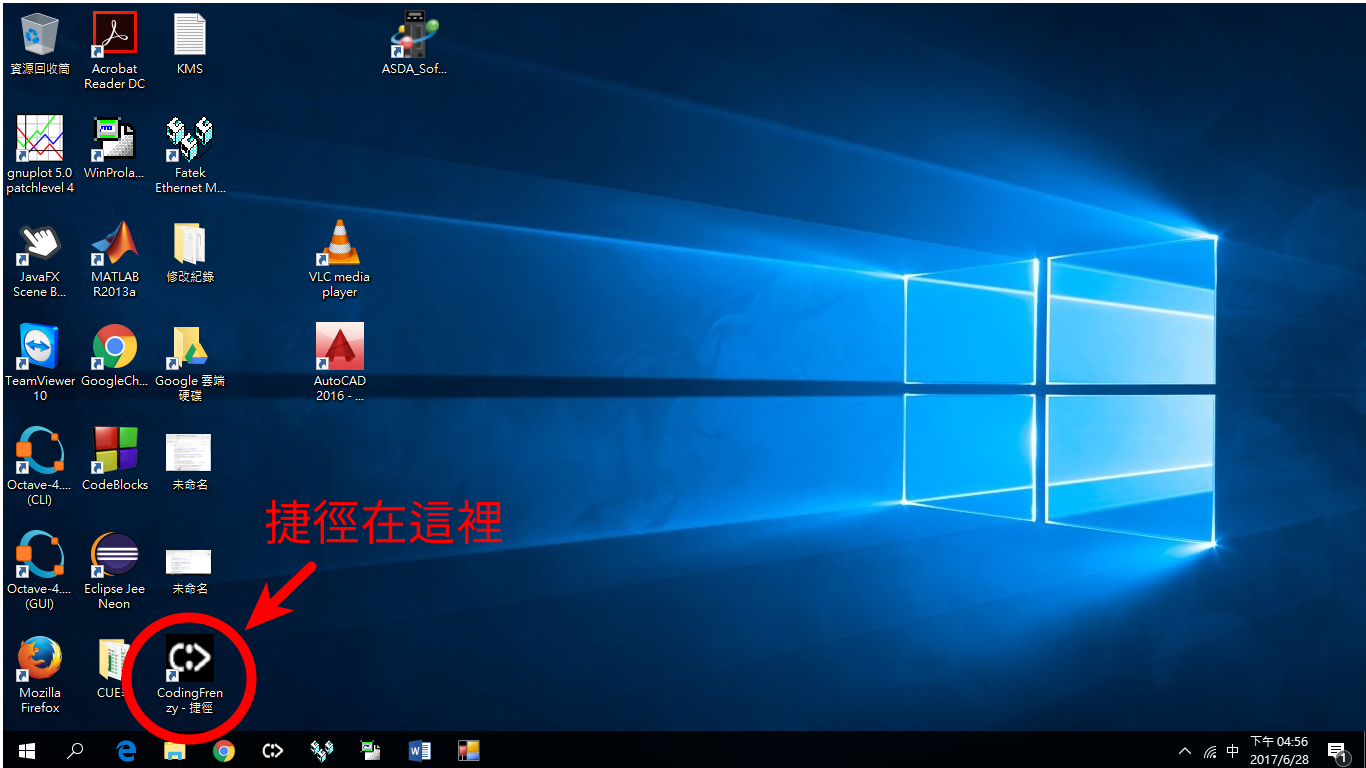
\includegraphics[width=0.8\textwidth]{fig/install_and_setting/install_024}
			\caption{桌面捷徑建立成功}
			\label{install024}
		\end{figure}

\newpage
\subsection{註冊瘋狂程設的帳號}
現在要教同學如何註冊瘋狂程設的帳號。網頁版及桌面版的瘋狂程設皆可註冊,方法大同小異,範例是使用網頁版進行註冊。

進入\href{http://coding-frenzy.arping.me/}{「瘋狂程設」}首頁後,點選左下角的「現在註冊一個帳戶吧!」,參考\autoref{register001}。
\begin{figure}[H]
	\centering
	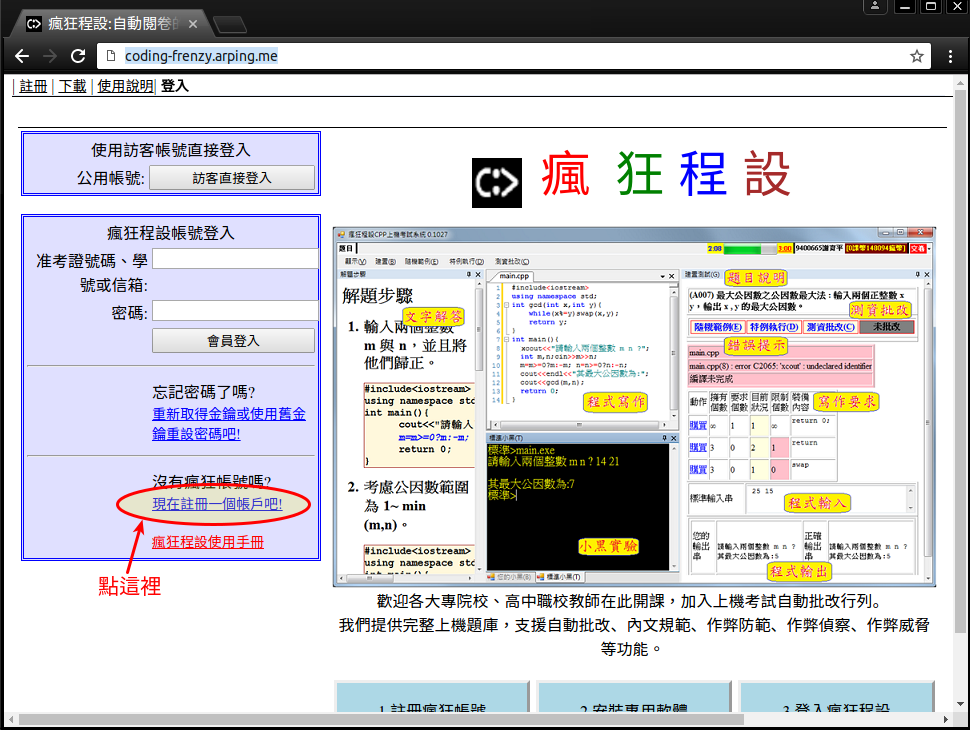
\includegraphics[width=0.8\textwidth]{fig/install_and_setting/register_001}
	\caption{註冊新帳戶}
	\label{register001}
\end{figure}

在框框處輸入你的電子信箱,完成後,按下方的按鈕「取得帳號金鑰」,參考\autoref{register002}。

註冊成功會顯示紅字「註冊成功,請前往信箱提取開頭為xxxx的金鑰來設定密碼。」,參考\autoref{register003}。
\begin{figure}[H]
	\centering
	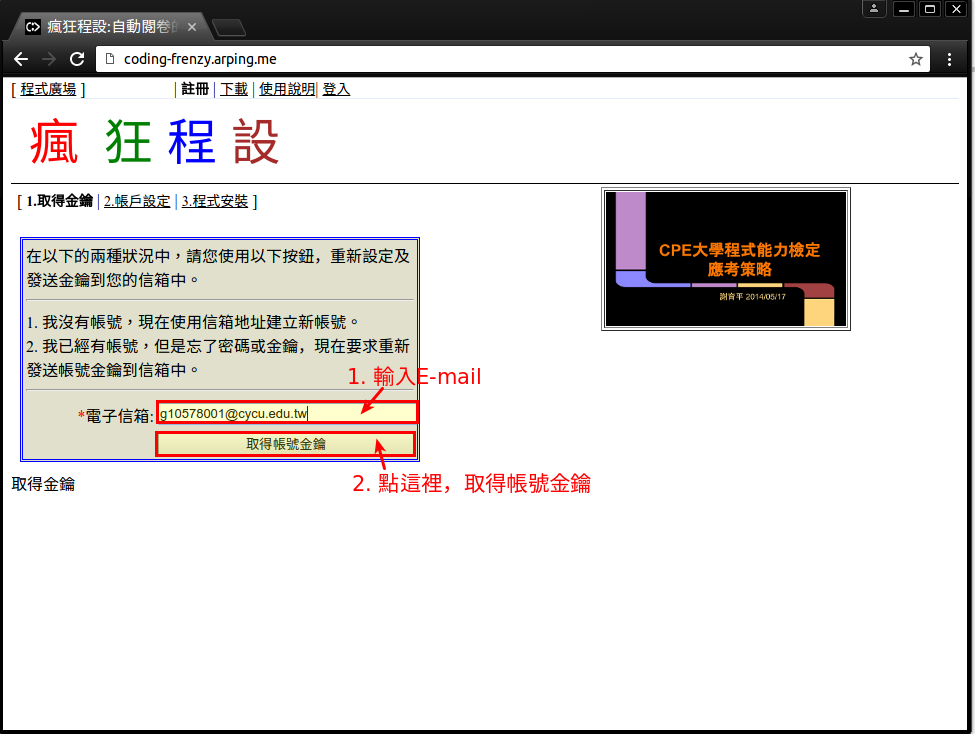
\includegraphics[width=0.8\textwidth]{fig/install_and_setting/register_002}
	\caption{輸入e-mail,取得金鑰}
	\label{register002}
\end{figure}



※範例中的金鑰開頭四碼是e017,你的金鑰開頭四碼與範例不同是正常的。
\begin{figure}[H]
	\centering
	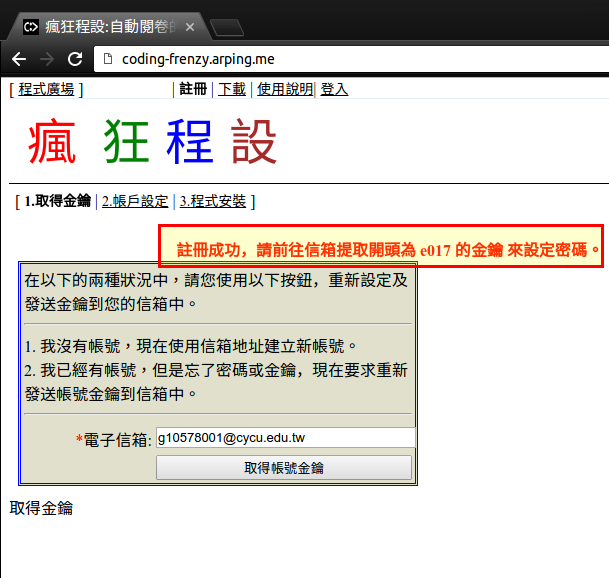
\includegraphics[width=0.7\textwidth]{fig/install_and_setting/register_003}
	\caption{成功取得金鑰}
	\label{register003}
\end{figure}

到你的電子信箱去收信,會收到一封主旨為「Coding-Frenzy Account is Created」的信,若沒收到可以去垃圾信件夾找找看,參考\autoref{register004}。
\begin{figure}[H]
	\centering
	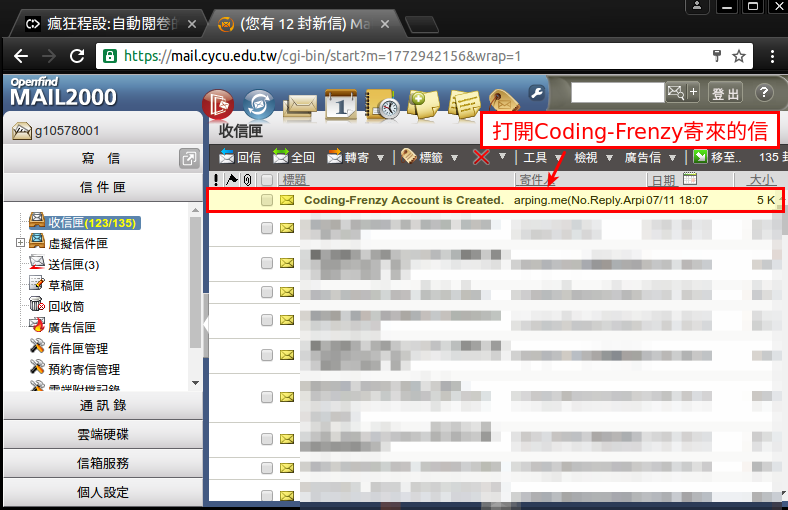
\includegraphics[width=0.8\textwidth]{fig/install_and_setting/register_004}
	\caption{去你的電子信箱收信}
	\label{register004}
\end{figure}

點LINK後面的連結,會自動開啟一個新的分頁,進入「帳戶設定」頁面,參考\autoref{register005}。
\begin{figure}[H]
	\centering
	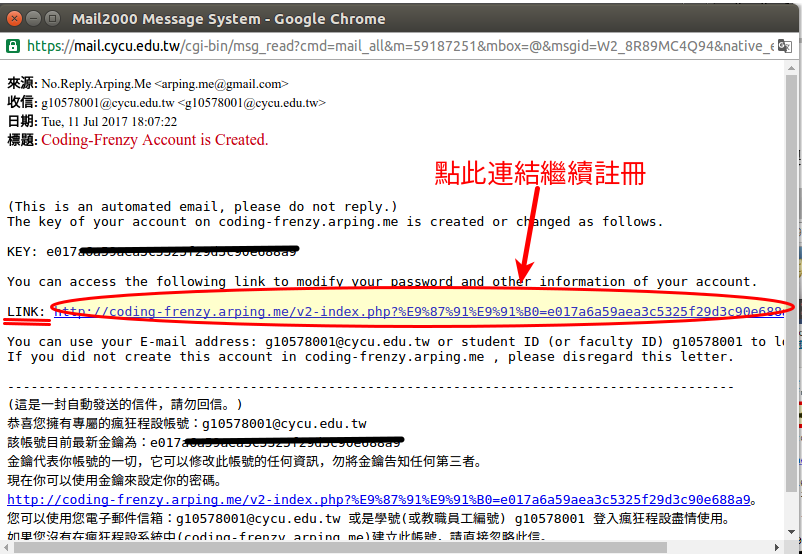
\includegraphics[width=0.8\textwidth]{fig/install_and_setting/register_005}
	\caption{點LINK後面的連結}
	\label{register005}
\end{figure}

\newpage
系統會自動填寫金鑰,將個人資料填寫完畢後,按下「我同意修改資料,並放棄個資法的求償權利。」,參考\autoref{register006}。

\begin{figure}[H]
	\centering
	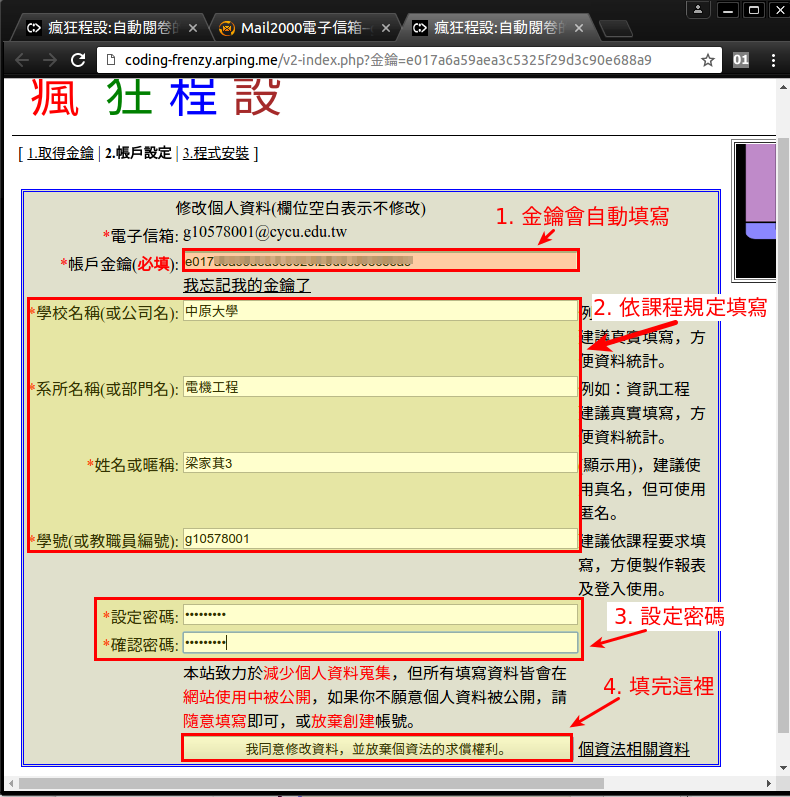
\includegraphics[width=0.9\textwidth]{fig/install_and_setting/register_006}
	\caption{填寫基本資料}
	\label{register006}
\end{figure}

\newpage
按下按鈕後,畫面沒有變化是正常的,這時候請先「登出」(頁面上方),參考\autoref{register007}。
\begin{figure}[H]
	\centering
	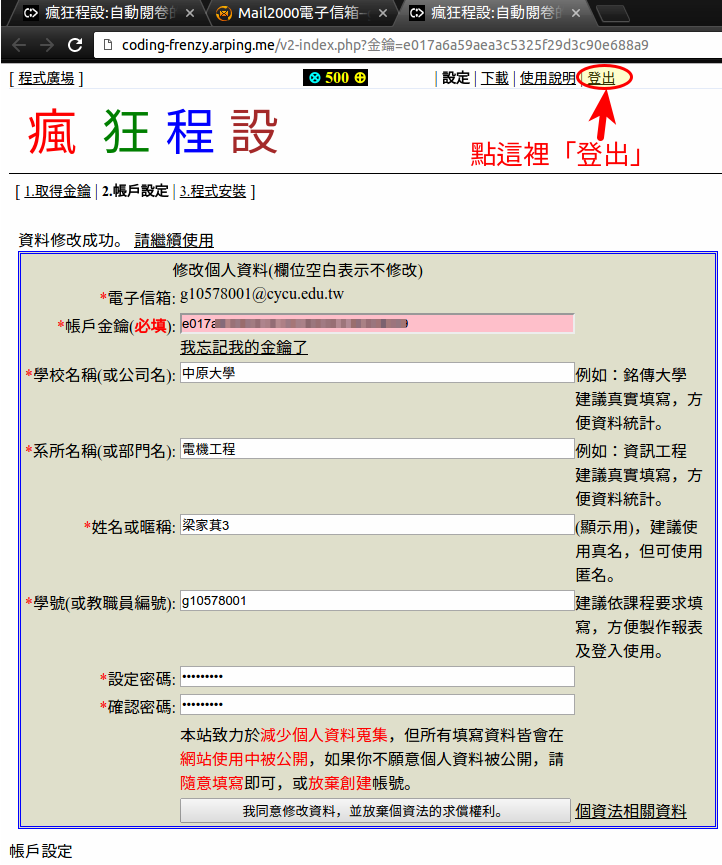
\includegraphics[width=0.9\textwidth]{fig/install_and_setting/register_007}
	\caption{登出}
	\label{register007}
\end{figure}

回到首頁後,用剛剛設定的學號及密碼登入,參考\autoref{register008}。

若看到此畫面,恭喜你完成註冊,參考\autoref{register009}。

\begin{figure}[H]
	\centering
	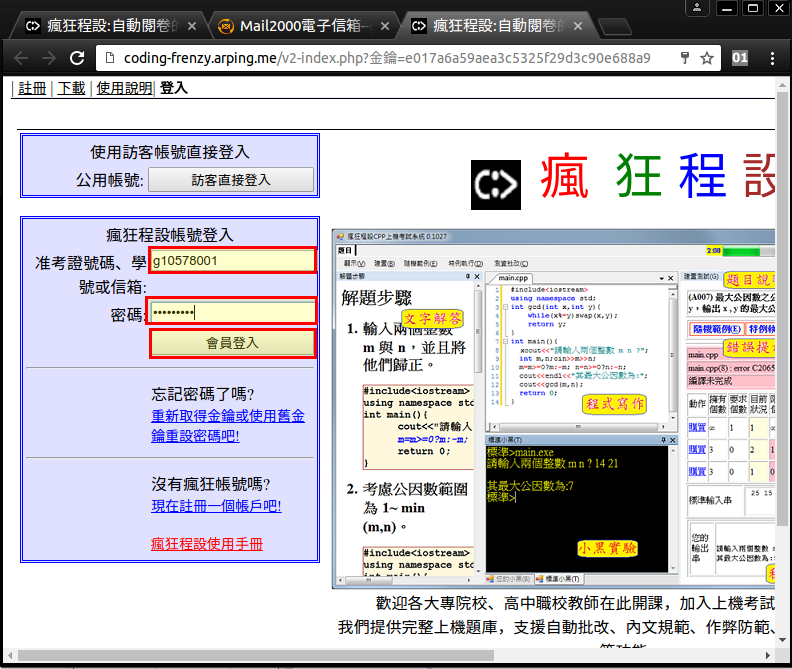
\includegraphics[width=0.8\textwidth]{fig/install_and_setting/register_008}
	\caption{登入畫面}
	\label{register008}
\end{figure}



\begin{figure}[H]
	\centering
	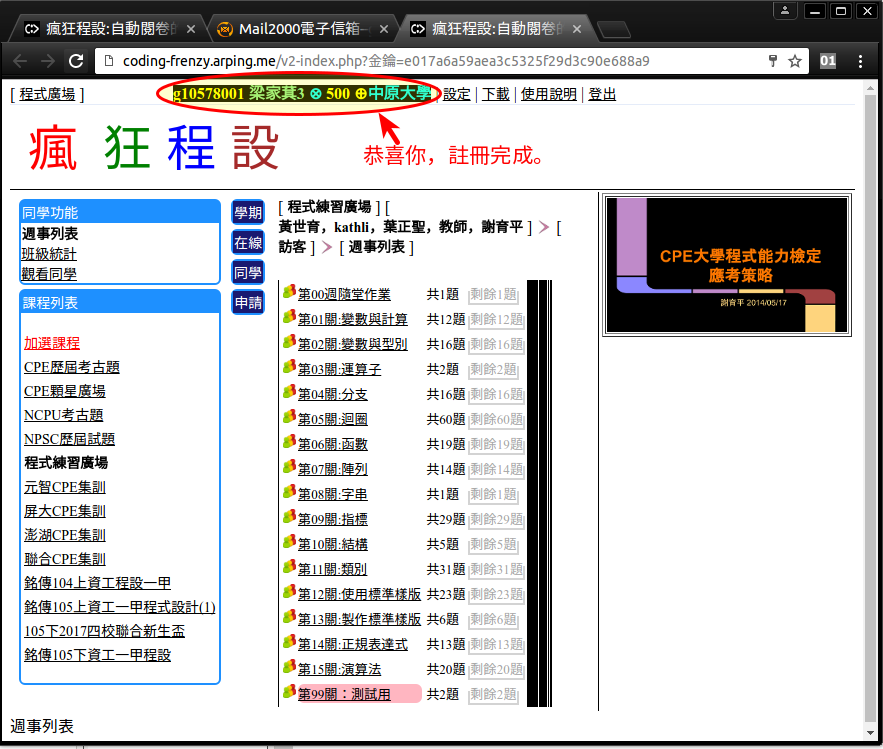
\includegraphics[width=0.8\textwidth]{fig/install_and_setting/register_009}
	\caption{登入成功}
	\label{register009}
\end{figure}

\subsection{如何使用瘋狂程設}
現在要說明如何使用瘋狂程設練習寫程式。

\begin{enumerate}
\item 點擊「程式練習廣場」。
\item 點擊「第01關:變數與計算」。
\item 點擊「練習」A001:Hello World。

參考\autoref{use001}。
\begin{figure}[H]
	\centering
	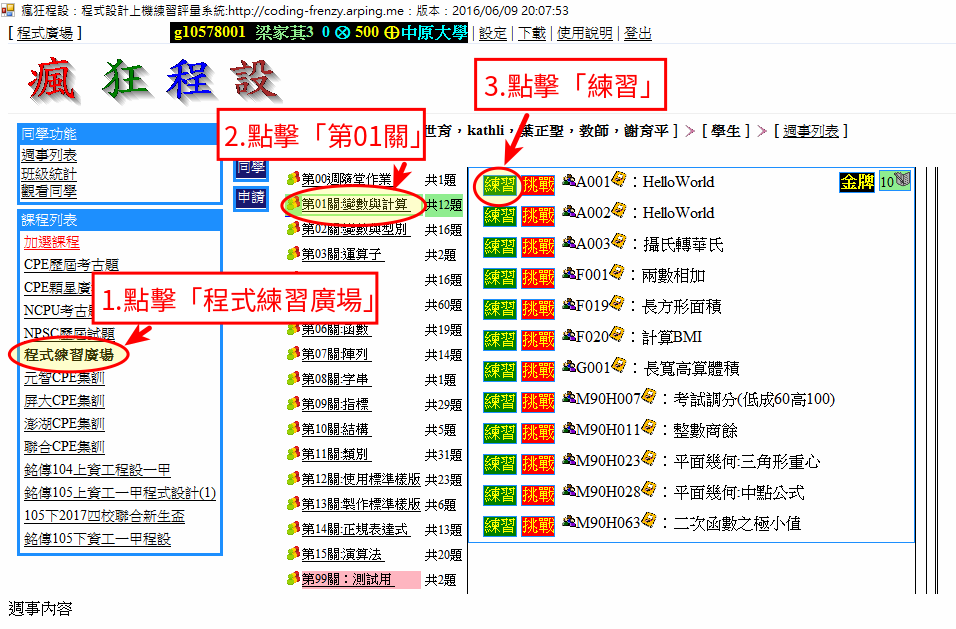
\includegraphics[width=0.8\textwidth]{fig/install_and_setting/use_001}
	\caption{選擇練習題目}
	\label{use001}
\end{figure}


\item 查看「題目資料」。
\item 有些題目的「解文」會有解題步驟。
\item 輸入程式碼。

注:程式碼的解說會在後續章節詳細說明,現在請直接照圖片上的範例輸入程式碼,或是複製「解文」裡的程式碼。

參考\autoref{use002}。
\begin{figure}[H]
	\centering
	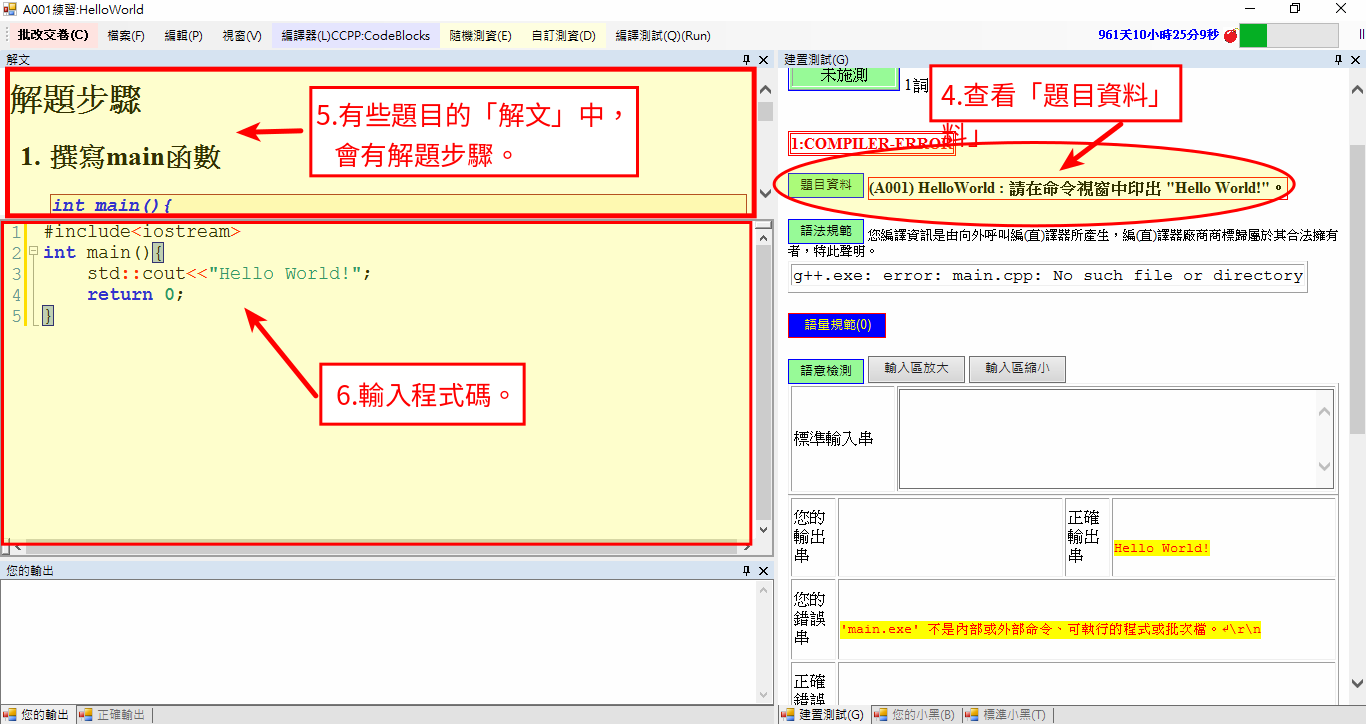
\includegraphics[width=0.8\textwidth]{fig/install_and_setting/use_002}
	\caption{依題目要求輸入程式碼}
	\label{use002}
\end{figure}


\item 設定「編譯器」,選擇「CCPP:CodeBlocks」,如果找不到此編譯器,請重新安裝CodeBlocks。

參考\autoref{use003}。
\begin{figure}[H]
	\centering
	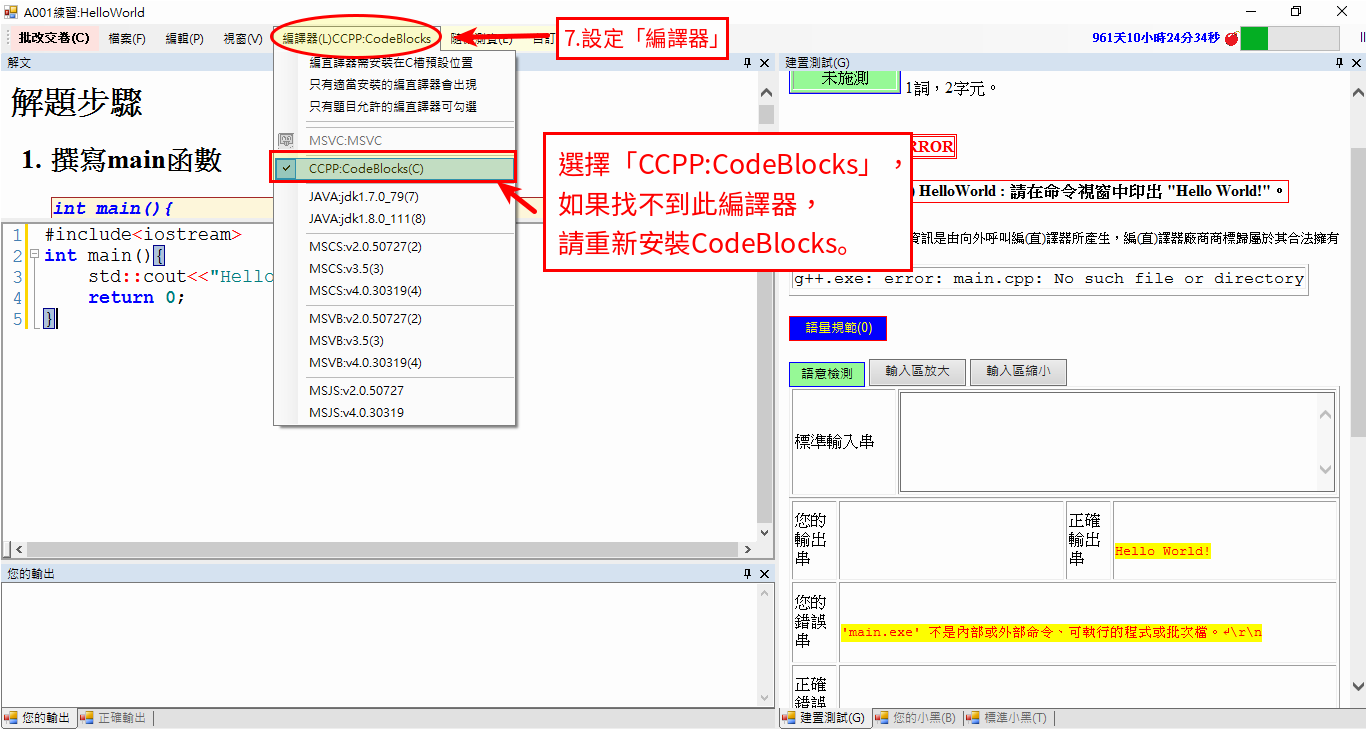
\includegraphics[width=0.8\textwidth]{fig/install_and_setting/use_003}
	\caption{設定「編譯器」}
	\label{use003}
\end{figure}


\item 點擊「隨機測資」或「自訂測資」。
\item 如果程式有錯誤。
\item 查看「編譯錯誤訊息」。

參考\autoref{use004}。
\begin{figure}[H]
	\centering
	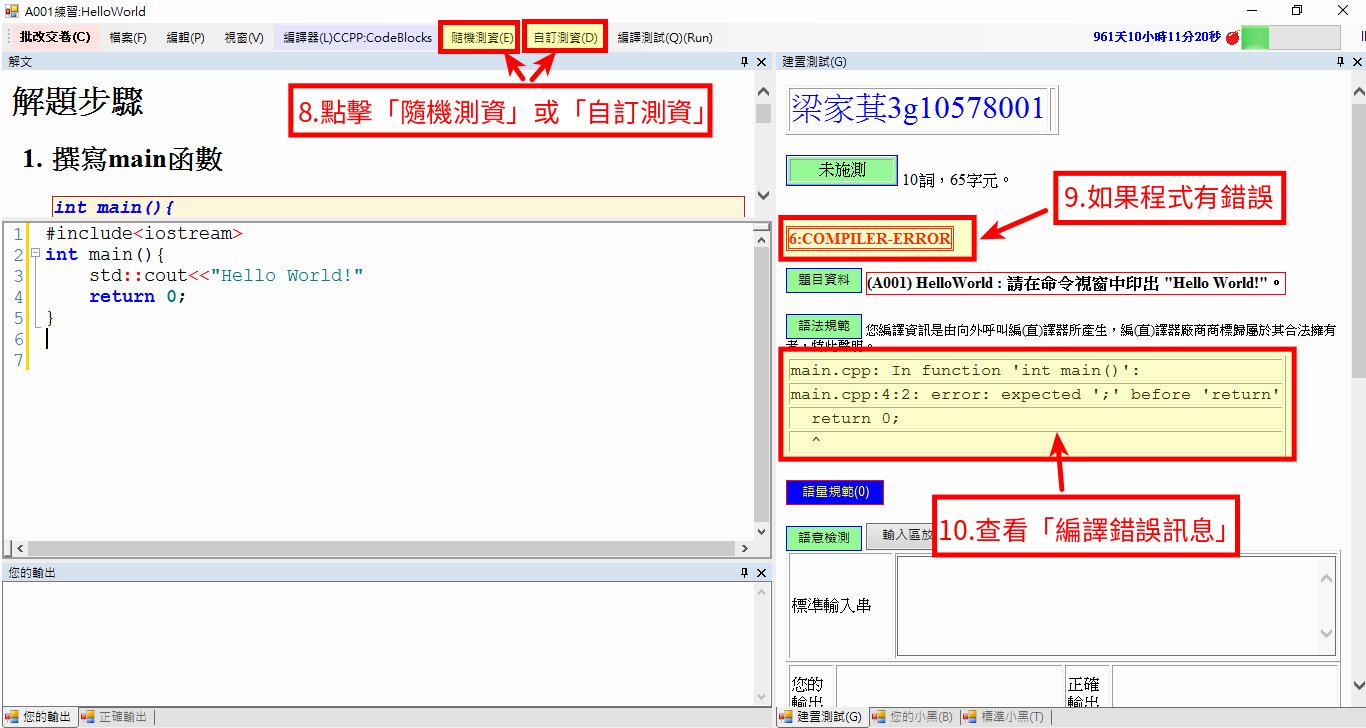
\includegraphics[width=0.8\textwidth]{fig/install_and_setting/use_004}
	\caption{測試程式碼}
	\label{use004}
\end{figure}


\item 修改程式碼。
\item 再次使用測資測試。
\item 程式正確,「顯示CORRECT」。
\item 點擊「批改交卷」。
\item 點擊「確定」,關閉提示視窗。
\item 顯示「通過」。
\item 關閉作答視窗。

參考\autoref{use005}。
\begin{figure}[H]
	\centering
	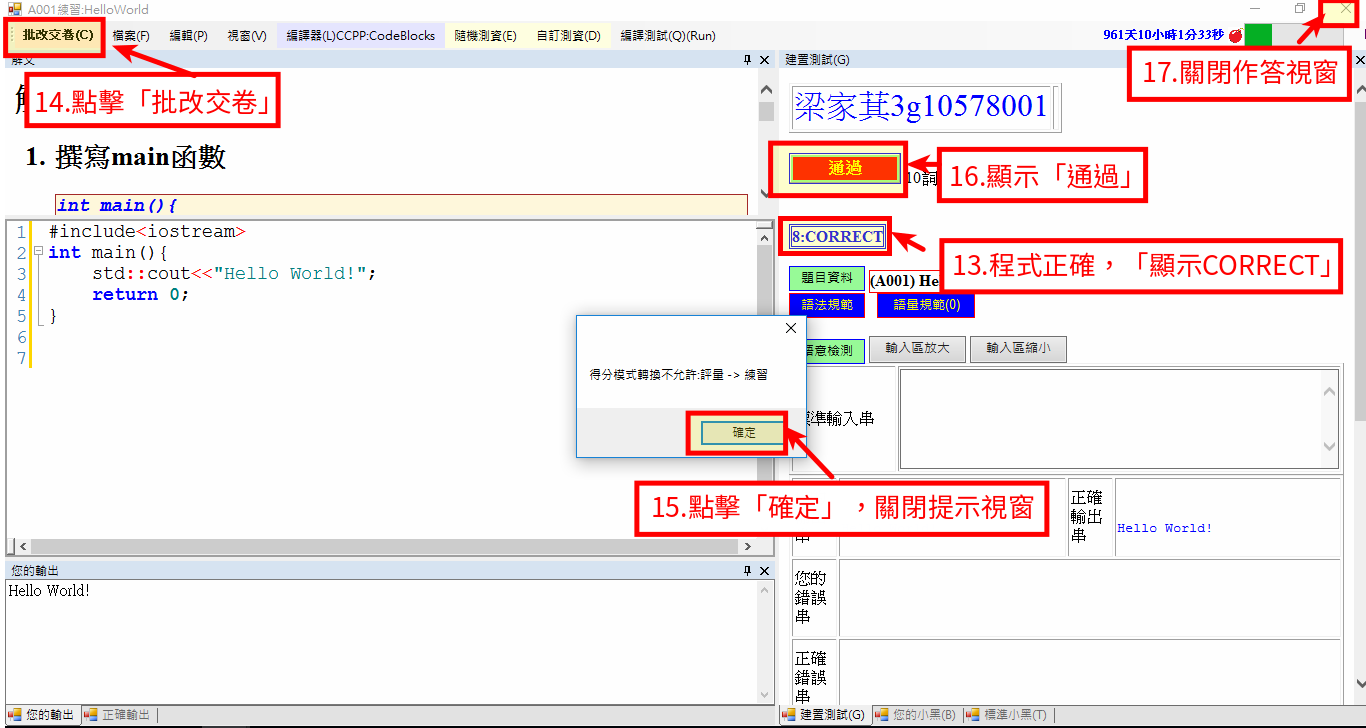
\includegraphics[width=0.8\textwidth]{fig/install_and_setting/use_005}
	\caption{批改交卷}
	\label{use005}
\end{figure}


\item 在主畫面按【F5】更新作答成績。
\item 通過「挑戰」模式,顯示「金牌」。
\item 通過「練習」模式,顯示「練習」。

參考\autoref{use006}。
\begin{figure}[H]
	\centering
	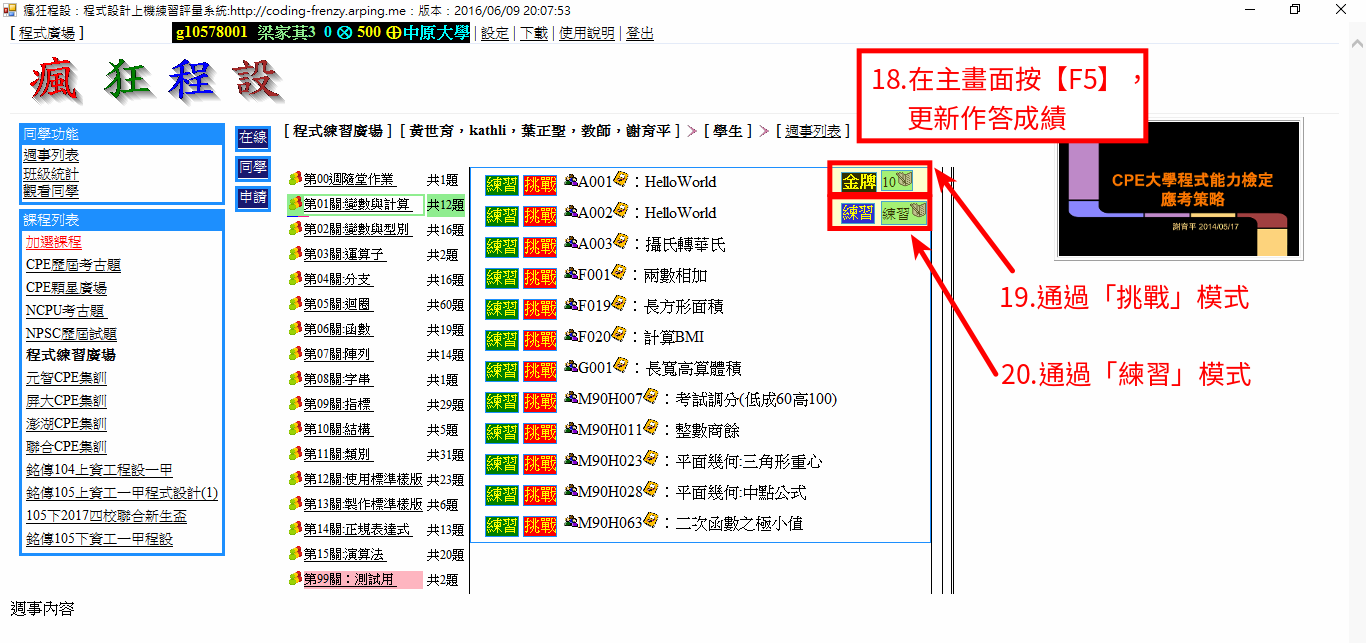
\includegraphics[width=0.8\textwidth]{fig/install_and_setting/use_006}
	\caption{查看成績}
	\label{use006}
\end{figure}

\end{enumerate}
